\chapter{The CMS detector at the LHC}
\label{label: chapDetector}

{\bf The LHC overview}

The Large Hadron Collider (LHC), as shown in
Figure~\ref{fig:LHC}, is the world$'$s largest and most powerful particle accelerator. 
It is a big underground ring of ${\approx}2.7$~km in circumference, sitting on the border of France and Switzerland. 
Inside the ring, the two high-energy proton beams are guided by the 
magnetic force, and then collide head-to-head in the 
positions of the four detectors: CMS, ATLAS, LHCb, ALICE. 

%{\color{red} Let's talk about a little bit about the beam}
At LHC, each proton beam has ${\approx}2000$ bunches and each bunch has $10^{11}$ protons. 
There is one bunch crossing (collisions of bunches) every 25~ns. The
large collision energy, the enormous amount of collisions and 
especially the large rate of bunch crossing
raise a big challenge for detecting the events after the collisions. 
%The design purpose
%of CMS detector is to discover new physics with a more accurate measurement. 

\begin{figure}[!htbp]
\centering
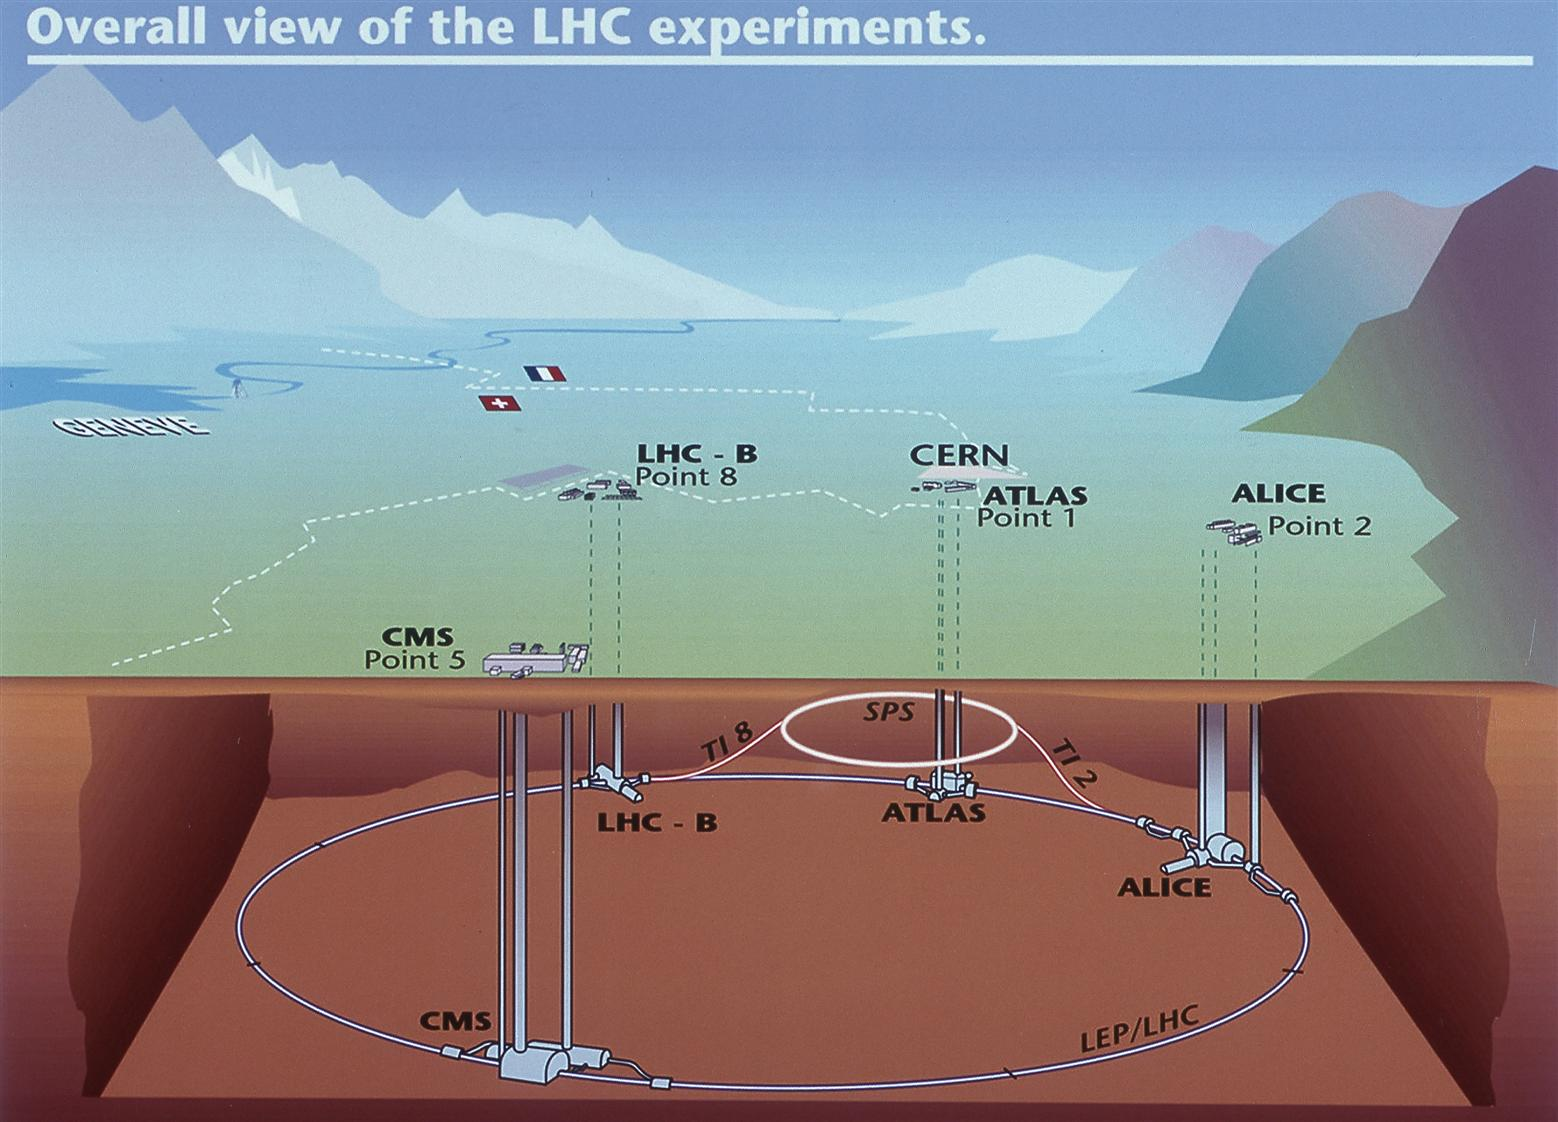
\includegraphics[width=.7\textwidth]{figures/CERN-LHC.jpg}
\caption{An overview of the LHC~\cite{LHC}.}
\label{fig:LHC}
\end{figure}

 
The focus of this chapter is to present a brief overview of the Compact Muon Solenoid (CMS) detector. 
Before that, the coordinate system of CMS is first introduced. 

{\bf The coordinate system of CMS}

In CMS, the z-axis is the along the beam line. The y-axis is vertically upward and the x-axis is directed 
radially inward the center of the LHC ring. As shown in Figure~\ref{fig:CMS_Slice}, the beam line, which is the z-axis, is perpendicular into this paper. And the x- and y-axes are on this paper but perpendicular to each other. 

\begin{figure}[!htbp]
\centering
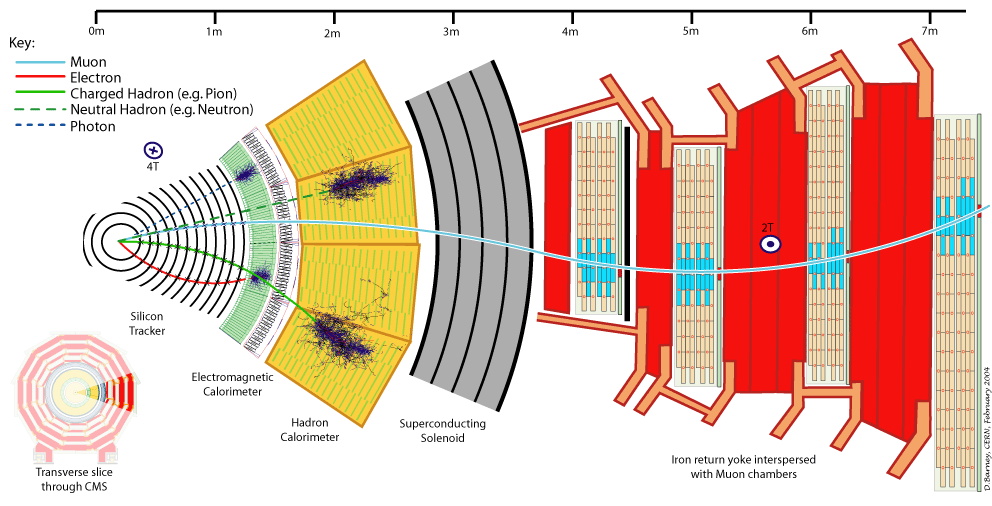
\includegraphics[width=.9\textwidth]{figures/CMS_Slice.png}
\caption{Transverse picture of the CMS detector.}
\label{fig:CMS_Slice}
\end{figure}


The default CMS x-y-z coordinate system and also the r-$\theta$-$\phi$ coordinate system are both right-handed. In the transverse plane (x-y plane), which is shown in Figure~\ref{fig:CMS_Slice},  the azimuthal angle 
$\phi$ is defined as the angle measured from the x-axis (${\rm tan}\phi = y/x$). And the transverse momentum $\pt$ is defined as $\pt = \sqrt{p_x^2 +p_y^2}$.  The polar angle $\theta$ is defined with respect to the the positive z-axis (${\rm tan}\theta = \sqrt{x^2+y^2}/z$).


The pseudorapidity $\eta$, as shown in Figure~\ref{fig:pseudo} is defined as $\eta = -{\rm ln}~{\rm tan}\big[\frac{\theta}{2}]$. And the rapidity is defined as $y = \frac{1}{2} {\rm ln} \frac{E+p_zc}{E-p_zc}$.  

\begin{figure}[!htbp]
\centering
\includegraphics[width=.9\textwidth]{figures/pseudorapidity.png}
\caption{The pseudorapidity $\eta$ and the $\theta$~\cite{wiki2}.}
\label{fig:pseudo}
\end{figure}


{\bf The CMS detector overview}

Along the beam line of LHC, there are four detectors: CMS, ATLAS, LHCb, ALICE. 
CMS is short for Compact Muon Solenoid, which indicates its profession in muon detecting. 
The overall layout of CMS from different view points are shown in Figure~\ref{fig:CMS_Slice} and Figure~\ref{fig:CMSLayout}. 
In Figure~\ref{fig:CMS_Slice}, the z axis is perpendicular into this paper. In Figure~\ref{fig:CMSLayout}, the z axis is on this paper, though the 
center of the detector.

The dimensions of the CMS detectors are a length of 21.6 m, a diameter of 14.6 m and a total weight of 12500 tons.  
From the beam line to the outside exterior, which is exactly from the left hand to the right hand of
Figure~\ref{fig:CMS_Slice}, there are silicon tracker, Electromagnetic Calorimeter, Hadronic Calorimeter, SuperConducting Solenoid,  Muon stations. 


\begin{figure}[!htbp]
\centering
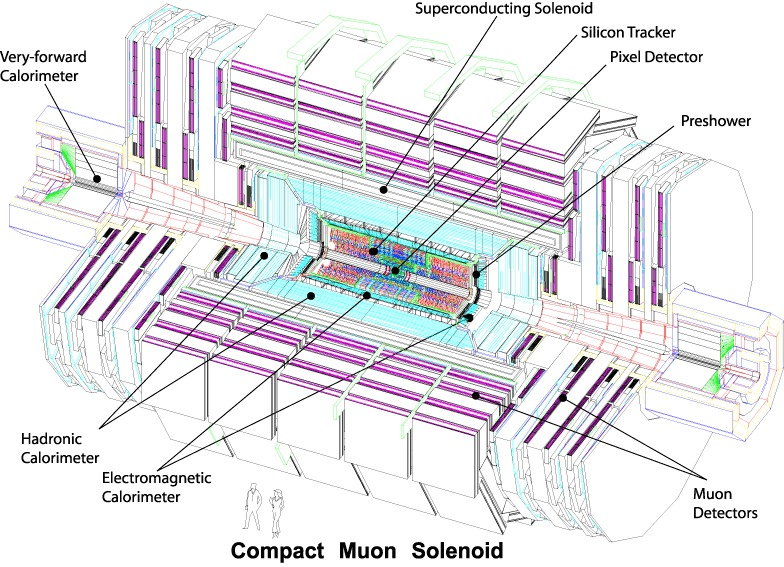
\includegraphics[width=.7\textwidth]{figures/cms_complete_layout.jpg}
\caption{An exploded view of the CMS detector.}
\label{fig:CMSLayout}
\end{figure}





%\section{The beam: luminosity and cross-section}

\section{The Magnet}

Each beam of LHC has 4~TeV energy in 2013, and it will reach 6.5~TeV in 2015, and 7~TeV in 2016. 
Particles from such energetic collisions are likely to have high $\pt$. 
So in CMS, to achieve a larger bending power of the high-$\pt$ charged particles, thus to get a
better momentum resolution, a large magnetic field of 4~T is chosen. 
In classical Electromagnetism, for a current of 1~Ampere in a loop of radius 3~m, the 
resulting magnetic field is ${\approx}10^{-7}$~T. So in CMS, to generate a field of 4~T for a radius of 
${\approx}3$~m, as shown in Figure~\ref{fig:CMS_Slice}, a super large current 19.5~kA is applied, with 2168 turns of coil. CMS solenoid uses a high-purity aluminium-stabilised conductor and indirect cooling by thermosyphon to achieve superconducting. 

The radius of the CMS solenoid is chosen to be large enough to accommodate the inner tracker and the calorimetry inside. The detailed parameters of this are shown in Table~\ref{table:magnet}.  

\begin{table}[htb]
\setlength{\tabcolsep}{12pt}
\caption{Parameters of the CMS superconducting solenoid.}
\begin{center}
\begin{tabular}{ cc }
Characteristics & Values \\
\hline
Field           &  4 T \\
Inner Bore  &  5.9 m \\
Length        &  12.9 m \\
Number of turns &  2168 \\
Current   &        19.5 kA  \\
Store energy &  2.7 GJ \\
Hoop stress   &   64 atm \\
\hline
\end{tabular} 
\end{center}
\label{table:magnet}
\end{table}

\section{The inner tracking system}

%{\color{red} Here we need a plot of the tracker layout and also the pixel tracker. If we could find a good description of the strip detector. }
As shown in Figure~\ref{fig:CMS_Slice}, the particles resulting from the collision point first pass through the silicon tracking detector. As we mentioned earlier, the enormous amount of collisions will produce a huge particle flux. For the tracker system, beside the challenge of radiation damage, the responsive time should be very fast and also the space resolution should be very accurate. These two 
aspects are the main design targets of the silicon tracker system. Here the overview and also details of the silicon tracker system are presented. 

The overall tracking volume is given by a cylinder of length of 5.8 m and diameter of 2.6 m. It is mainly
composed of two parts: the inner pixel tracker and the layers of the outer strip tracker.    

Three layers of silicon pixel detectors are placed closed to the interaction region to improve the measurement of impact parameter \footnote{The details about what impact parameter is could be found : \url{http://en.wikibooks.org/wiki/LaTeX/Footnotes_and_Margin_Notes}} of charged-particle tracks, as well as the position of secondary vertices. 
In addition, CMS uses 10 layers of silicon microstrip detector, which provide the required granularity and precision.  
The detailed layout of the tracker system is shown in Figure~\ref{fig:trackerLayout}. 

\begin{figure}[!htbp]
\centering
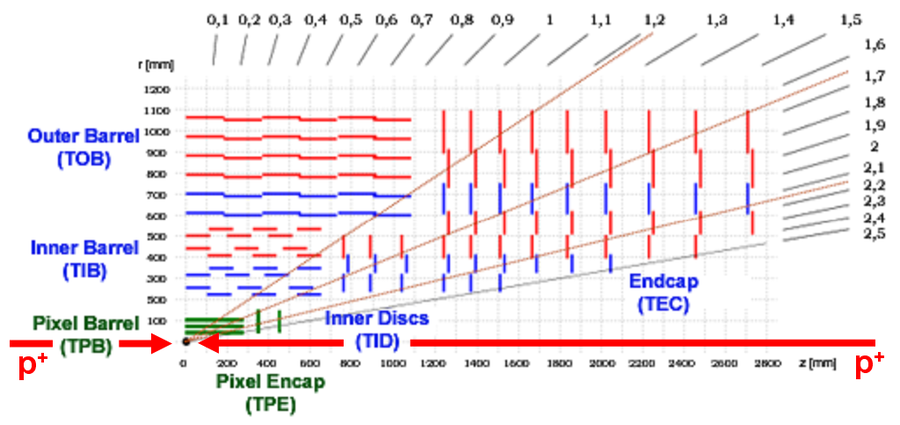
\includegraphics[width=0.8\textwidth]{figures/TrackerLayout.png}
\caption{The tracker layout of CMS.}
\label{fig:trackerLayout}
\end{figure}

{\bf The pixel detector}

Close to the interaction vertex, in the barrel region, are 3 layers of hybrid pixel detectors at a radii of 4.4, 7.3, and 10.2 cm, which is about the size of a shoe box, as shown in Figure~\ref{fig:pixel}. 
Each layer is spilt into sensor segments like mosaic tiles. Each silicon sensor, with the size of $100 \times 150~(\mu m)^2$, is about two hairs' widths.
The endcap of pixel detector is composed of two disks of pixel modules on each side of the barrel region, extending from 6 to 15~cm in radius. 

\begin{figure}[!htbp]
\centering
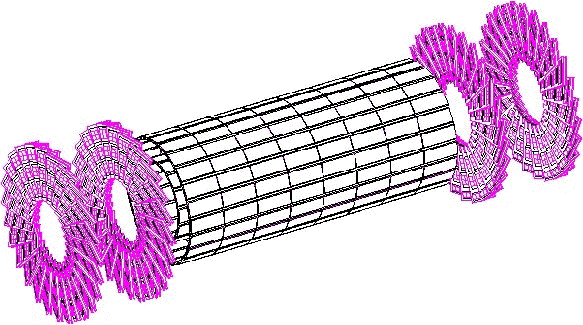
\includegraphics[width=0.8\textwidth]{figures/pixel.png}
\caption{Layout of the pixel detector in the CMS~\cite{expBook}.}
\label{fig:pixel}
\end{figure}

When a charge particle passes trough the sensor, 
it raises an electronic signal. 
Knowing which pixels have been passed allows us to reconstruct the charged particle$'$s trajectory. 
Because the pixel detector is made of 2D tiles,  and has three layers,  a three-dimensional picture of the particle's motion is created.
The spatial resolution of the pixel detector is ${\approx}10~ \mu m$ for the $r{-}\phi$ measurement and
${\approx}20~\mu m$ for the $z$ measurement. 





{\bf The strip detector}

After passing through the three pixel layers, particles travel through ten layers of silicon strip detectors, 
as shown in Figure~\ref{fig:Strip}, which reaches out to a radius of 130~cm. The silicon strip tracking detector consists of four inner barrel (TIB) layers assembled in shells with two inner endcaps (TID), each composed of three small discs. The outer barrel (TOB) consists of six concentric layers. Finally two endcaps (TEC) close off the tracker. Each part of the strip detector has silicon modules designed differently for its place within the detector.

\begin{figure}[!htbp]
\centering
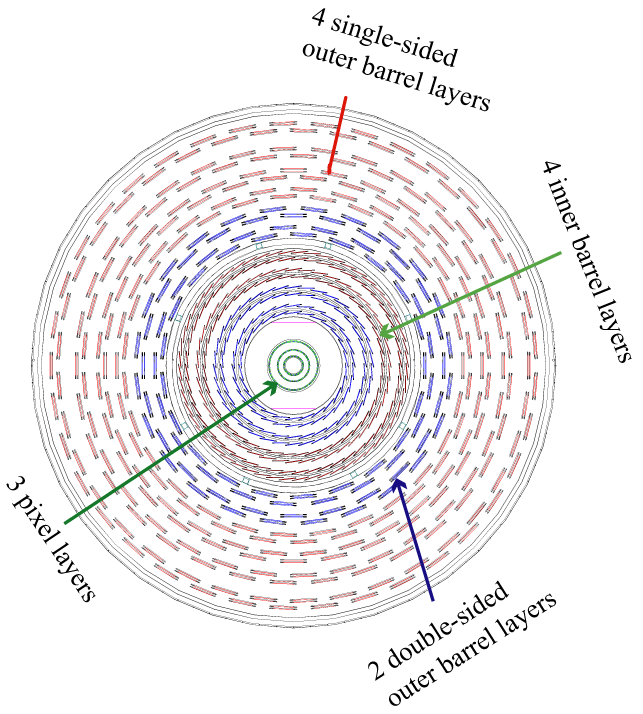
\includegraphics[width=0.8\textwidth]{figures/Strip.png}
\caption{Layout of tracker system of CMS, with z-axis perpendicular into the paper.}
\label{fig:Strip}
\end{figure}


Unlike the 2D pixel sensor, most of the 10 strip layers are composed of 1D strip sensors. So when a charged particle passes through the strip sensor, the strip detector only outputs the local 1D position instead of 2D position. 
%The design purpose for strip detector is to provide additional particle tracks for the inner pixel detectors. 
%Combined information of the pixel and strip detectors will provide 



\section{Electromagnetic calorimeter (ECAL) }



The ECAL is designed to calibrate the energy of electron and photons resulting from proton-proton (pp) collisions at LHC, and its structure is shown in Figure~\ref{fig:ECAL}.  
ECAL uses lead tungstate (${\rm PbWO_4}$) crystals with coverage in $|\eta|$ up to 3.0. 
The lead tungstate crystal is highly transparent and ``scintillates'' when electrons and photons pass through it, which produces light in proportion to the charged particles$'$ energy. It also has short radiation (0.89~cm) and Moliere (2.2~cm) lengths, and is fast and radiation hard. However, 
the ${\rm PbWO_4}$ crystal produces relatively low light yield.
%Beside all the good characteristics that lead tungstate has short radiation (0.89 cm) and Moliere (2.2 cm) lengths, are also fast and radiation hard, it produces relatively low light yield. 
So the silicon avalanche photodiodes (APDs), which could amplify the light signal into electric signal, are used as photodetectors in the ECAL barrel (EB) and 
vacuum phototriodes (VPTs) in the ECAL endcap (EE). 
 
 
\begin{figure}[!htbp]
\centering
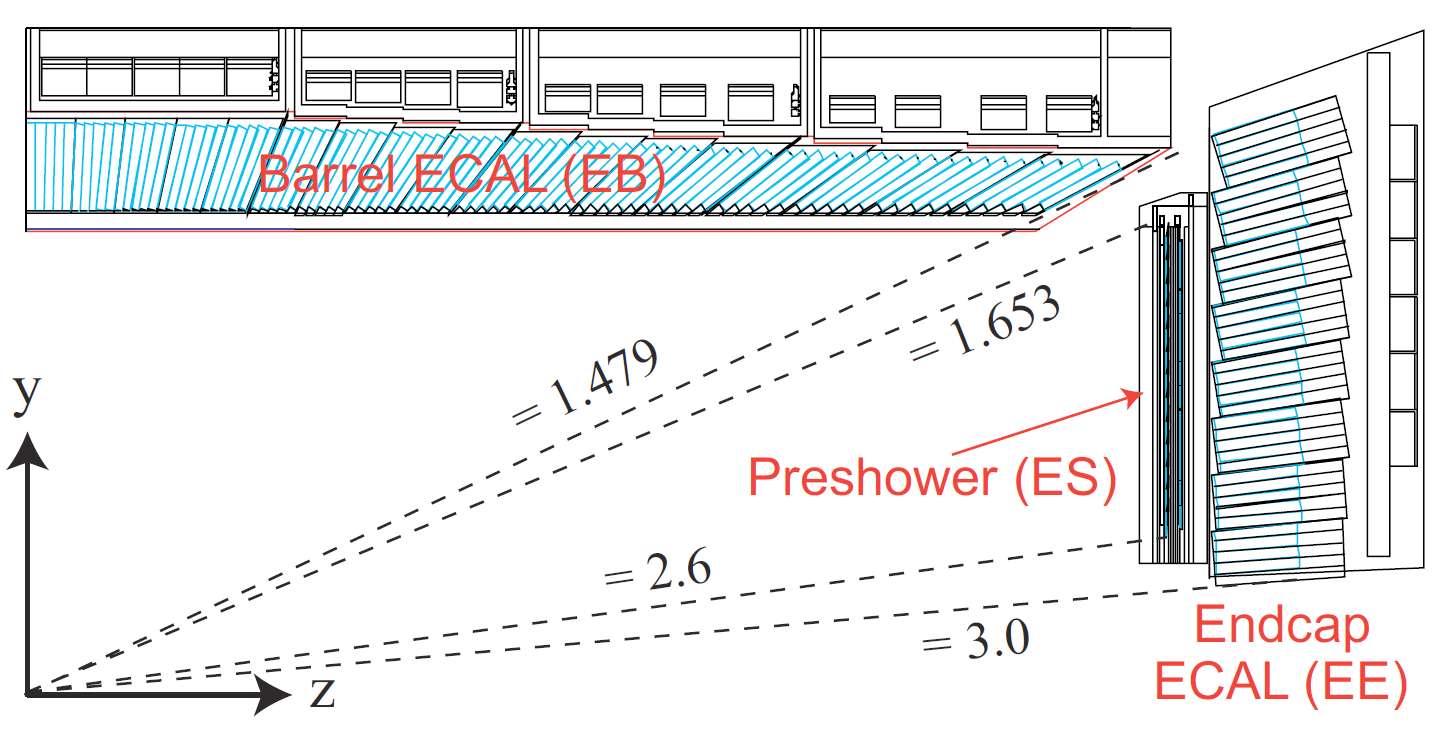
\includegraphics[width=.8\textwidth]{figures/ECALEta.png}
\caption{Geometric view of one quarter of the ECAL.}
\label{fig:ECAL}
\end{figure}

  
These photodetectors have been especially designed to work within the high magnetic field. They are glued onto the back of each of the crystals to detect the scintillation light and convert it to an electrical signal that is amplified and sent for analysis.
 
 A preshower system is installed in front of the EE.  
The preshower is made of two planes of lead followed by silicon sensors. 
%, similar structure to those used in the tracker.  
The reason for the preshower system is that short-lived particles called neutral pions, produced in pp collisions, can inadvertently mimic high-energy photons when they decay into two closely-spaced lower energy photons that the ECAL picks up together. And for Higgs discovery,
the high energy photons from Higgs decay is the important signature of $H \to \gamma \gamma$ channel. So the preshower system could identify the photons from neutral pion decay and distinguish them from the photons of $H \to \gamma \gamma$  decay.
  

  \section{Hadronic calorimeter (HCAL)}
  
%  ECAL is surrounded by a brass/scintillator sampling hadron calorimeter with coverage up to $|\eta| < 3.0$. 
HCAL is designed to measure the energy of hadrons and also the transverse
missing energy $E_{T}^{miss}$. Improving the energy resolution and achieving good hermeticity for
the the $E_{T}^{miss}$ measurement, are the two main goals of HCAL design. 
 
As shown in Figure~\ref{figs:HCAL},  HCAL is composed by four parts, HCAL barrel (HB), HCAL endcap (HE), HCAL outer (HO) and HCAL forward (HF).  HF, not presented in the plot, sits on the outside of the muon stations and covers $3 <  |\eta| < 5.0$.  

Brass is the filling material of HCAL.  
It is chosen because it is non-magnetic and has short interaction length. To achieve a good containment, HCAL maximizes the brass inside of the solenoid by
minimizing the detection material with the application of the tile/filbre technology~\cite{expBook}. HCAL is a sample detector, in which layers of brass are interleaved by layers of fibre. 
The HO is located outside of the solenoid, to complement the measurement of HB. 

 
\begin{figure}
\centering
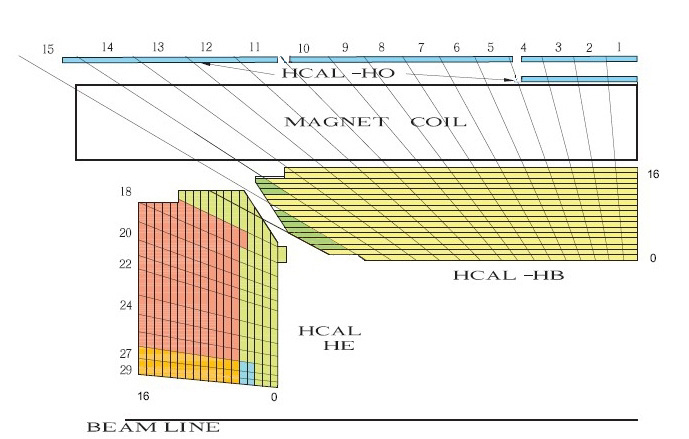
\includegraphics[width=.8\textwidth]{figures/Hcal.jpg}
\caption{Geometric view of one quarter of the HCAL.}
\label{figs:HCAL}
\end{figure}
  
  
\section{Muon system}
%CMS is called the "compact muon solenoid". Muon detecting at CMS is very important. 

The layout of one quarter of the CMS muon system for the initial low luminosity running is shown in 
Figure~\ref{fig:Muonsystem},  and the transverse view of the muon stations (MSs) is shown in 
Figure~\ref{fig:MuonStation}, with z-axis perpendicular into the paper. In 
Figure~\ref{fig:MuonStation}, the red colored part is the return yoke, which has a magnetic field of
2~T. As shown in Figures~\ref{fig:Muonsystem} and~\ref{fig:MuonStation},  in the Muon Barrel (MB) region, 4 stations of detectors are arranged in cylinders interleaved with the iron yoke.   
This magnetic field in the return yoke bends the trajectory of muon, while there is almost no magnetic field in the 
four muons stations (MS1, MS2, MS3, MS4). In the adjacent muon stations by comparing the bending angle because of the return yoke , the muon system correctly calculates the muon momentum. 

\begin{figure}
\centering
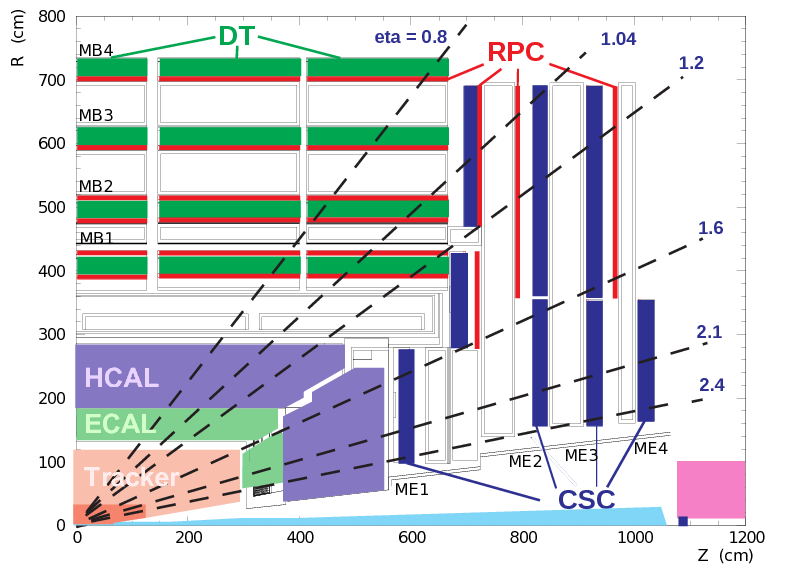
\includegraphics[width=.8\textwidth]{figures/Muonsystem.png}
\caption{Layout of one quarter of the CMS muon system for initial low luminosity running. The 
RPC system is limited to $|\eta| < 1.6$ in the endcap, and for the CSC system only the inner ring of the ME4 chambers  have been deployed.}
\label{fig:Muonsystem}
\end{figure}

\begin{figure}
\centering
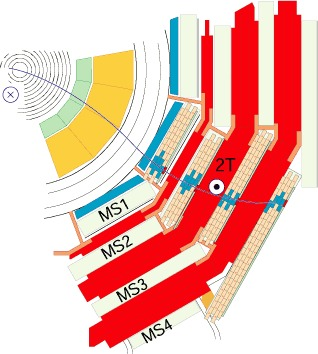
\includegraphics[width=.8\textwidth]{figures/MuStations.jpg}
\caption{The Muon stations in the transverse view. }
\label{fig:MuonStation}
\end{figure}
  

From Figure~\ref{fig:Muonsystem}, three types of gaseous detectors are used to identify and measure muons: drift tube (DT), cathode strip chamber (CSC), and resistive plate chamber (RPC). 

Drift tube (DT), with detailed layout in Figure~\ref{fig:DT}, is used in the barrel region ( $|\eta| < 1.2$).  In this region, the residual magnetic field in the chambers is low and also muon rate is low, so drift tube is chosen. When a muon or any charged particle passes through the gas volume, it knocks electrons off the atoms of the gas. These electrons follow the electric field ending up at the 
positively-charged wire (anode wire in Figure~\ref{fig:DT}). By registering where in the wire and also the time the electrons take to reach the wire, the DT could provide a 2D position of the passing charged particle.  
The maximum drift length is 2.0 cm and the single point resolution is $\approx$ 200 $\mu m$.
 
\begin{figure}[!htbp]
\centering
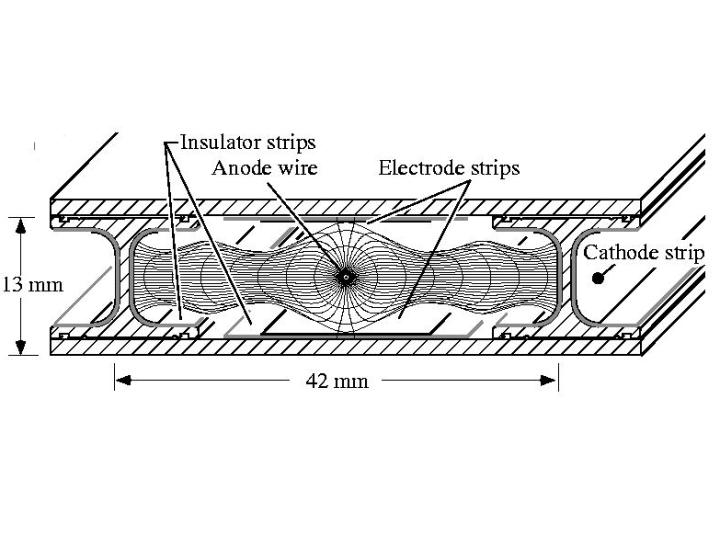
\includegraphics[width=.8\textwidth]{figures/DriftTubeDetails.jpg}
\caption{Layout of the drift tube~\cite{web:DT}.}
\label{fig:DT}
\end{figure} 
 
In the endcap region,  cathode strip chambers (CSCs) are used because of the high residual magnetic field and also high muon rate. As shown in Figure~\ref{fig:CSC}, 
CSCs consist of arrays of positively-charged ``anode'' wires crossed with negatively-charged copper ``cathode'' strips within a gas volume. When muons pass through, they knock electrons off the gas atoms, which flock to the anode wires producing an avalanche of electrons. Positive ions move away from the wire and towards the copper cathode, also inducing a charge pulse in the strips, at 
the right angles to the wire direction.
Because the strips and the wires are perpendicular, we get two position coordinates for each passing charged particle.

\begin{figure}[!htbp]
\centering
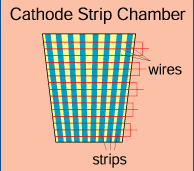
\includegraphics[width=.8\textwidth]{figures/CSC.png}
\caption{Layout of the drift tube~\cite{web:CSC}.}
\label{fig:CSC}
\end{figure} 


In addition to this, resistive plate chambers (RPCs), as shown in Figure~\ref{fig:RPC}, are used in both the barrel and the endcap regions. The RPCs could provide a fast response with a good time resolution but with a coarser position resolution than the DTs and the CSCs.  So the RPCs could identify the correct bunch crossing (25~ns per bunch crossing). 

\begin{figure}[!htbp]
\centering
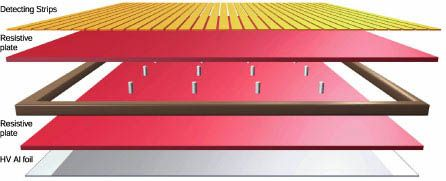
\includegraphics[width=.8\textwidth]{figures/RPC.jpg}
\caption{Layout of the resistive plate chamber~\cite{web:CSC}.}
\label{fig:RPC}
\end{figure}

Muons from pp collisions are measured 3 times: in the silicon tracking system, after the solenoid coil, and in the muon chambers (the muon system). 
Measurement of the momentum of muons using only the muon system, is essentially determined by the muon bending angle when it exits  the 4~T solenoid, taking the interaction point of pp collision as the origin of the muon.
For low-momentum muons, the best momentum resolution is given by the resolution 
obtained in the silicon tracker. For high-momentum muons, combining the inner tracker and muon detector measurements will highly improve the muon momentum resolution.  
At CMS, in $0 < |\eta| < 2.0 $, for $\mu$ with $\pt$ $200{\sim}400$ GeV ,  $\Delta p / p$ is measured to be $\leq 3\%$.


\section{Trigger and data acqusition}

As mentioned earlier, there is one bunch crossing per 25~ns. While for each bunch crossing, there 
is ${\approx}40$ millions pp collisions. Although the readout of CMS is fast enough, it costs a lot to store 
this amounts of events. So CMS adopts a two-level trigger system to filter out the uninteresting events. 

The Level-1 (L1) trigger is automatic and universally applied to each event, with the application of hardware processors. Basically, L1 trigger sets a threshold for ``trigger primitive" objects, like photon, muon, electron, and jets to be above some $E_{T}$ or $p_{T}$.  After the L1 trigger, the event rate reduces to 100~kHz. 

The L2 trigger, which is also named as high level trigger (HLT), is used to further reduce the 100~kHz to 
100 Hz event rate. 
In L2 trigger system, the event from pp collision is partially reconstructed. 
Information about the calorimeter and muons is first reconstructed and compared with the threshold of L2. Events falling this threshold will be immediately thrown out. Then information of pixel tracks is reconstructed and tested with the corresponding threshold. Following this kind of process, without reconstructing all possible objects in an event, L2 is more flexible and has complete freedom in selecting events. 

Data, after the trigger system, is fully reconstructed, and taped on the disks. 
%L-2 trigger first reconstructs the calorimeter and muon information, and test the threshold of them, immediately 
%throw out non-interesting events. Then L2 partially reconstruct the pixel tracking information, and throw out non-interesting events.  Following this process,  without reconstructing all possible objects in an event, the software-based L2 trigger is more flexible and has complete freedom in selecting events. 
  









  



  



 
 
 





